\documentclass[a4paper,10pt,twoside]{article}

\usepackage[top=1in, bottom=1in, left=1in, right=1in]{geometry}
\usepackage[utf8]{inputenc}
%\usepackage[spanish,es-ucroman,es-noquoting]{babel}
\usepackage{fancyhdr}
\usepackage{lastpage}
\usepackage{graphicx}



%%%%%%%%%% Configuración de Fancyhdr - Inicio %%%%%%%%%%
\pagestyle{fancy}
\thispagestyle{fancy}
\lhead{TP1, Sistemas Operativos}
\renewcommand{\footrulewidth}{0.4pt}
\cfoot{\thepage /\pageref{LastPage}}

\fancypagestyle{caratula} {
   \fancyhf{}
   \cfoot{\thepage /\pageref{LastPage}}
   \renewcommand{\headrulewidth}{0pt}
   \renewcommand{\footrulewidth}{0pt}
}

%%%%%%%%%% Macros de tikz - Fin %%%%%%%%%%


\begin{document}


%%%%%%%%%%%%%%%%%%%%%%%%%%%%%%%%%%%%%%%%%%%%%%%%%%%%%%%%%%%%%%%%%%%%%%%%%%%%%%%
%% Carátula                                                                  %%
%%%%%%%%%%%%%%%%%%%%%%%%%%%%%%%%%%%%%%%%%%%%%%%%%%%%%%%%%%%%%%%%%%%%%%%%%%%%%%%


\thispagestyle{caratula}

\begin{center}


\includegraphics[height=2cm]{DC.png} 
\hfill

\includegraphics[height=2cm]{UBA.jpg} 

\vspace{2cm}

Departamento de Computación,\\
Facultad de Ciencias Exactas y Naturales,\\
Universidad de Buenos Aires

\vspace{4cm}

\begin{Huge}
TP1 - Scheduling
\end{Huge}

\vspace{0.5cm}

\begin{Large}
Sistemas Operativos
\end{Large}

\vspace{1cm}

Primer Cuatrimestre de 2015

\vspace{4cm}

\vspace{0.5cm}

\begin{tabular}{|c|c|c|}
\hline
Apellido y Nombre & LU & E-mail\\
\hline
Cisneros Rodrigo		& 920/10 & rodricis@hotmail.com\\
Rodr\'iguez, Agust\'in	& 120/10 & agustinrodriguez90@hotmail.com\\
Tripodi, Guido			& 843/10 & guido.tripodi@hotmail.com\\
\hline
\end{tabular}

\end{center}

\newpage


%%%%%%%%%%%%%%%%%%%%%%%%%%%%%%%%%%%%%%%%%%%%%%%%%%%%%%%%%%%%%%%%%%%%%%%%%%%%%%%
%% Índice                                                                    %%
%%%%%%%%%%%%%%%%%%%%%%%%%%%%%%%%%%%%%%%%%%%%%%%%%%%%%%%%%%%%%%%%%%%%%%%%%%%%%%%


\tableofcontents

\newpage


%%%%%%%%%%%%%%%%%%%%%%%%%%%%%%%%%%%%%%%%%%%%%%%%%%%%%%%%%%%%%%%%%%%%%%%%%%%%%%%
%% Introducción                                                              %%
%%%%%%%%%%%%%%%%%%%%%%%%%%%%%%%%%%%%%%%%%%%%%%%%%%%%%%%%%%%%%%%%%%%%%%%%%%%%%%%


\section{Introducción}

\indent \indent En este Trabajo Práctico estudiaremos diversas implementaciones de algoritmos de scheduling. 
Haciendo uso de un simulador provisto por la cátedra podremos reprensentar el comportamiento de estos algoritmos. 
Implementaremos dos Round-Robin, uno que permite migración de tareas entre núcleos y otro que no y a través de experimentación intentaremos comparar ambos algoritmos. 
Asimismo, basándonos en un paper implementaremos una versión del algoritmo para scheduler con prioridades
dinámicas y otro para prioridades estáticas y 
mediante experimentos intentaremos comprobar ciertas propiedades que cumplen los algoritmos desarrollados.\\

%%%%%%%%%%%%%%%%%%%%%%%%%%%%%%%%%%%%%%%%%%%%%%%%%%%%%%%%%%%%%%%%%%%%%%%%%%%%%%%
%% Desarrollo                                                                %%
%%%%%%%%%%%%%%%%%%%%%%%%%%%%%%%%%%%%%%%%%%%%%%%%%%%%%%%%%%%%%%%%%%%%%%%%%%%%%%%

\newpage
\section{Desarrollo y Resultados}

\section{Parte I – Entendiendo el simulador simusched}


\subsection{Ejercicios}
\begin{itemize}
 \item \textbf{Ejercicio 1 }
 En primer lugar, deberán implementar un Read-Write Lock libre de inanición utilizando únicamente Variables de Condición POSIX 
 y  respetando la interfaz provista en los archivos backend-multi/RWLock.h y backend-multi/RWLock.cpp
\end{itemize}

\subsection{Resultados y Conclusiones}

\subsubsection[Resolución Ejercicio 1]{Ejercicio 1}

\indent Nuestra implementación del Read-Write Lock se baso en el pseudocodigo implementado en el libro $The$ $Little$ $Book$ $of$ $Semaphores$
al resolver la inanición producida en el problema de $Readers-writers$.\\

Se utilizaron 3 Semaphores, los cuales son:\\
\begin{itemize}
 \item roomEmpty
 \item turnstile
 \item readers$\_$mutex
\end{itemize}

Y ademas, un entero denominado $readers$\\

Comenzando por la implementación de los lectores, el pseudocodigo del libro mencionado es el siguiente:\\

\begin{verbatim}
            turnstile.wait()
            turnstile.signal()

            readSwitch.lock(roomEmpty)
                # critical section for readers
            readSwitch.unlock(roomEmpty)
\end{verbatim}

De aquí nuestro código implementado fue el siguiente:\\

\begin{center}
            \textbf{READERS LOCK}     
\end{center}

 
\begin{verbatim}
            pthread_mutex_lock(&turnstile);
            pthread_mutex_unlock(&turnstile);

            pthread_mutex_lock(&readers_mutex);
            readers++;
            pthread_mutex_unlock(&readers_mutex);
\end{verbatim}

Como se puede observar en el codigo del lock del read, el lector realiza un lock (wait) y unlock (signal) del Semaphores $turnstile$
para tener su turno y que ningún otro lo saque.\\
Por consiguiente, se realiza el lock del mutex que se encuentra vinculado al entero $readers$, ya que este será
aumentará su cantidad en 1 para que de esta manera nadie pueda modificarlo, y luego es liberado dicho mutex ($readers\_mutex$).\\

Luego, nuestro $READ$ $UNLOCK$ fue el siguiente:\\

\begin{center}
            \textbf{READERS UNLOCK}
\end{center}

 
\begin{verbatim}
            pthread_mutex_lock(&readers_mutex);
            readers--;
            if (readers == 0) {
                pthread_cond_signal(&room_empty);		
            }
            pthread_mutex_unlock(&readers_mutex);
\end{verbatim}

En esta implementación, primero se realiza un lock del Semaphore vinculado al entero $readers$ ya que este disminuirá en 1.\\
Luego, se realiza una consulta chequeando el valor del entero, si este es 0 se le dara un signal al Semaphore $room\_empty$
para notificarle al escritor que ya no queda ningun lector y puede proceder a escribir.\\
Por último, se libera el mutex $readers\_mutex$.\\

Continuando con el escritor, el pseudocodigo fue el siguiente:\\

\begin{verbatim}

            turnstile.wait()
            roomEmpty.wait()
                # critical section for writers
            turnstile.signal()

            roomEmpty.signal()

\end{verbatim}

De aquí, nuestra implementación final fue:\\

\begin{center}
            \textbf{WRITERS LOCK}
\end{center}

 
\begin{verbatim}
            pthread_mutex_lock(&turnstile);
            pthread_mutex_lock(&readers_mutex);
            while(readers != 0)
                  pthread_cond_wait(&room_empty, &readers_mutex);
            pthread_mutex_unlock(&readers_mutex);
\end{verbatim}

Inicialmente en nuestra implementación del WRITE LOCK, se realiza un lock del Semaphore $turnstile$ para que nadie pueda quitarle el turno, se realiza un
lock del mutex vinculado al entero, y luego se ingresa a un ciclo siempre que $readers$ sea distinto de 0, esto se realiza
para luego poder ejecutar la funcion $pthread\_cond\_wait$ para que esta misma tenga un funcionamiento correcto y seguro al
chequear la condición sobre $room\_empty$.\\
Una vez que se salga del ciclo o no se ingrese al mismo se libera el mutex $readers\_mutex$.\\

Luego, la implementación del unlock fue:\\
\begin{center}
           \textbf{WRITERS UNLOCK}
\end{center}

 
\begin{verbatim}
           pthread_mutex_unlock(&turnstile);
\end{verbatim}

Para la implementación del unlock del writer solo se libera el Semaphore $turnstile$.\\

De esta manera, con dicha implementación, siempre que llegue un escritor el mismo tendrá su turno sin producirse inanición.
Ya que, en caso de haber lectores y llegar un escritor, estos terminaran de leer y en caso 
de llegar nuevos lectores deberán esperar a que el escritor finalice su ejecución.\\

\newpage
%\subsection{Filtro Miniature}

\section{Parte II: Extendiendo el simulador con nuevos schedulers}


\subsection{Ejercicios}
\begin{itemize}
 \item 
\textbf{Ejercicio 3}  Completar la implementación del scheduler Round-Robin implementando los
metodos de la clase SchedRR en los archivos sched rr.cpp y sched rr.h. La implementacion
recibe como primer parametro la cantidad de nucleos y a continuacion los valores de sus
respectivos quantums. Debe utilizar una unica cola global, permitiendo ası la migracion de
procesos entre nucleos.
\item \textbf{Ejercicio 4} Diseñar uno o mas lotes de tareas para ejecutar con el algoritmo del ejercicio
anterior. Graficar las simulaciones y comentarlas, justificando brevemente por que el comportamiento 
observado es efectivamente el esperable de un algoritmo Round-Robin.
\item \textbf{Ejercicio 5} A partir del articulo:\\
\begin{itemize}
 \item Liu, Chung Laung, and James W. Layland. Scheduling algorithms for multiprogramming
in a hard-real-time environment. Journal of the ACM (JACM) 20.1 (1973): 46-61.
\end{itemize}
1. Responda:
\begin{enumerate}
 \item ¿Que problema estan intentando resolver los autores?
 \item ¿Por que introducen el algoritmo de la seccion 7? ¿Que problema buscan resolver
con esto?
\item Explicar coloquialmente el significado del teorema 7.
\end{enumerate}
2. Diseñar e implementar un scheduler basado en prioridades fijas y otro en prioridades
dinamicas. Para eso complete las clases $SchedFixed$ y $SchedDynamic$ que se encuentran
en los archivos $sched$\_$fixed.[h|cpp]$ y $sched$\_$dynamic.[h|cpp]$ respectivamente.
\end{itemize}


\subsection{Resultados y Conclusiones}

\subsubsection[Resolución Ejercicio 3]{Ejercicio 3}
Para desarrollar la implementación del scheduler $Round-Robin$ y que este funcione de una forma correcta
utilizamos una serie de estructuras puntuales. \\
Las mismas son las siguientes:\\
\begin{enumerate}
 \item Una cola global, la cual nombramos $q$, esta contiene los $PID$ de los procesos activos que no estan
 bloqueados y en el tope de la misma se encuentra el próximo proceso a correr. Esta cola,
 fue desarrollada para que cuando se desaloje un proceso por finalizar su $quantum$ la misma pase al final de
 la cola y generando el ciclo acorde al comportamiento de este scheduler.
 \item Un vector denominado $cores$, este tiene en su elemento $i$ el pid correspondiente a
al proceso que está corriendo en el core $i+1$. Inicializamos todos los elementos en -1, esto
corresponde a la Idle Task, de esta forma reconocemos que no se cargaron procesos en los núcleos.
\item Un vector $quantum$ guarda en la posicion $i$ el quantum que se dispuso a cada núcleo.
\item Un vector $quantumActual$ aqui guardaremos la cantidad de ticks que le quedan al proceso
desde que fue cargado en el core.
\item Una lista de $bloqueados$ esta tendra procesos que se bloquearon cuando estaban corriendo.
\end{enumerate}

De esta manera, con estas estructuras nos permiten determinar para cada tarea, cuándo, y cuánto 
de su quantum consumieron de forma que podamos desalojarla correctamente.\\

A su vez, tomamos ciertas decisiones en esta implementación:
\begin{itemize}
 \item Si una tarea se encuentra bloqueada cuando se produce el tick del reloj, esta misma es desalojada
de la cola global, y agregada en un lista de bloqueados. Además, sera reseteado el quantum, se le
dará inicio a la próxima tarea que se encuentre ready y cuando el sistema operativo, nos envie una
señal de unblock, la tarea desalojada regresará al final de la cola global.

\end{itemize}


\subsubsection[Resolución Ejercicio 4]{Ejercicio 4}

\indent El algoritmo de scheduler \textbf{Round-Robin} tiene como caracter\'istica asignar a todas las tareas 
un determinado tiempo m\'aximo de procesamiento, a esto se lo llama $quantum$. \\
\indent Este tiempo esta definido para cada n\'ucleo en particular, dependiendo de en cu\'al de ellos est\'en 
ejecutando los procesos, se les asignar\'a el respectivo tiempo m\'aximo.\\
\indent Otra caracter\'istica del \textbf{Round-Robin} es que las tareas se encolan y se ejecutan c\'iclicamente. 
Osea que cuando se deja de ejecutar, si no termin\'o su ejecuci\'on, la tarea se encolar\'a al final de la lista. 
Como elecci\'on de diseño, elegimos que se use una cola global para todos los procesadores, aunque tambi\'en
se podr\'ia tener una cola para cada n\'ucleo. \\
\indent A su vez, tambi\'en puede ocurrir una tarea no consuma todo su $quantum$. 
Ya sea porque la tarea se bloquea (haciendo uso de dispositivos de entrada/salida) o porque termine su ejecuci\'on.\\
\indent En caso de haber terminado, nuestro algoritmo pone a correr directamente la pr\'oxima tarea de acuerdo al orden 
circular que se estableci\'o y la tarea que finaliz\'o se desalojar\'a por completo y no sera considerada nuevamente. \\
\indent En caso de haberse bloqueado, esta misma dejar\'a de ser considerada hasta que se desbloquee, 
perdiendo el quantum que le quedaba si hubiere. 
Autom\'aticamente, seguir\'a corriendo la pr\'oxima tarea que se encuentre en la cola global. 
Cuando el proceso se desbloquee, ser\'a encolada nuevamente al final de dicha cola.   \\

\indent Para corroborar que el comportamiento era el deseado, desarrollamos 3 disversos lotes de tareas compuestos por tareas
del tipo $taskConsola$ y $taskCpu$, trabajando con 1, 2 y 3 cores y utilizando el mismo $quantum$ para cada uno de los mismos.\\

Nuestro primer lote de tareas fue el siguiente:
\begin{verbatim}
                                     TaskCPU 70
                                     TaskConsola 2 4 5
                                     TaskCPU 40
                                     TaskConsola 3 2 3
                                     TaskCPU 30
\end{verbatim}

Obteniendo los siguientes resultados:

\begin{center}

    
	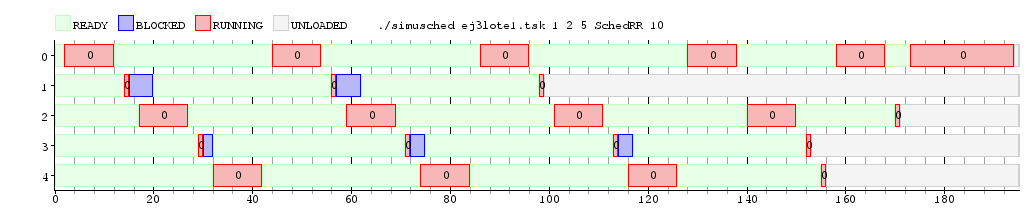
\includegraphics[width=450pt]{./EJ4_RR/ejercicio4-1nucleo.png}
	{$Lote 1$ - Scheduler RR - 1 core}	
 
\end{center}


\indent Con esta simulación, trabajamos con 2 ticks de cambio de contexto.\\
\\
\indent Se puede observar el cambio de tareas cíclico tanto porque terminaron su quantum o porque se bloquearon.\\

\begin{center}
  	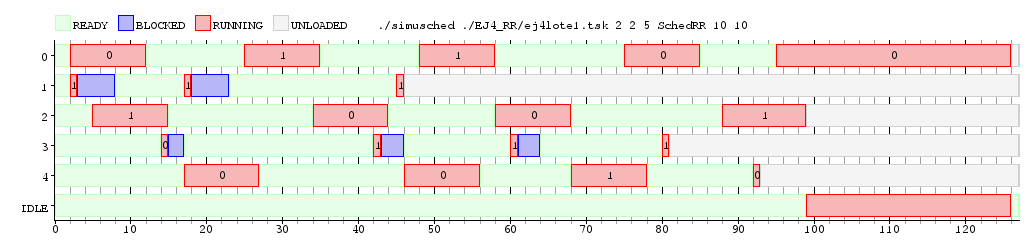
\includegraphics[width=450pt]{./EJ4_RR/ejercicio4-2nucleo.png}
	  {$Lote 1$ - Scheduler RR - 2 core}	
\end{center}

\begin{center}
  	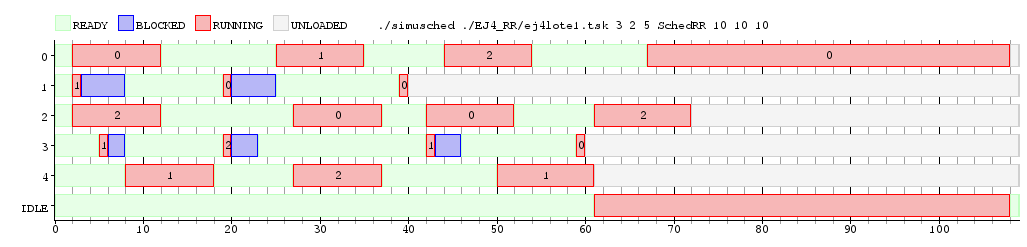
\includegraphics[width=450pt]{./EJ4_RR/ejercicio4-3nucleo.png}
	  {$Lote 1$ - Scheduler RR - 3 core}	
\end{center}

\indent Es notorio, ademas del la ejecuciòn circular de las tareas, un cierto paralelismo al estar trabajando con
2 o 3 cores.\\

\indent Luego, de esta simulación probamos con un lote con tareas que se bloqueen por más tiempo:
 \begin{verbatim}
                                     TaskCPU 70
                                     TaskConsola 5 6 7
                                     TaskCPU 40
                                     TaskConsola 10 9 8
                                     TaskCPU 30
 \end{verbatim}

\indent Manteniendo la misma cantidad de tick para cambio de contexto y core. También, nos parecio prudente, mantener
los mismos valores de $quantum$ obteniendo los siguientes gráficos:

\begin{center}
    	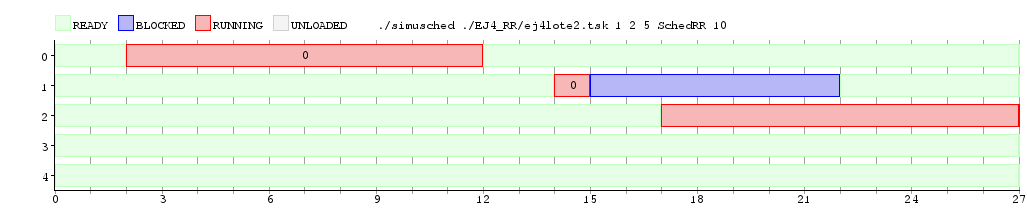
\includegraphics[width=450pt]{./EJ4_RR/ejercicio4-2lote1nucleo.png}
	{$Lote 2$ - Scheduler RR - 1 core}	
 \end{center}

 \begin{center}
    	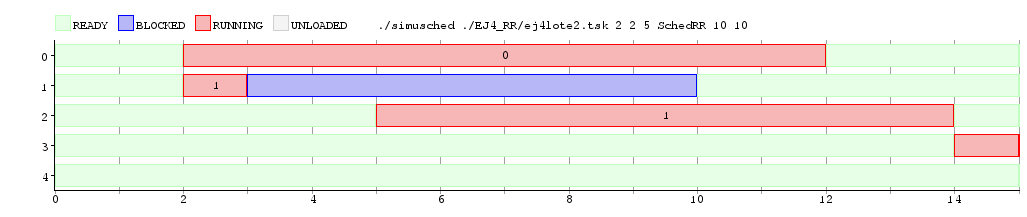
\includegraphics[width=450pt]{./EJ4_RR/ejercicio4-2lote2nucleo.png}
	{$Lote 2$ - Scheduler RR - 2 core}	
 \end{center}
 
 \begin{center}
    	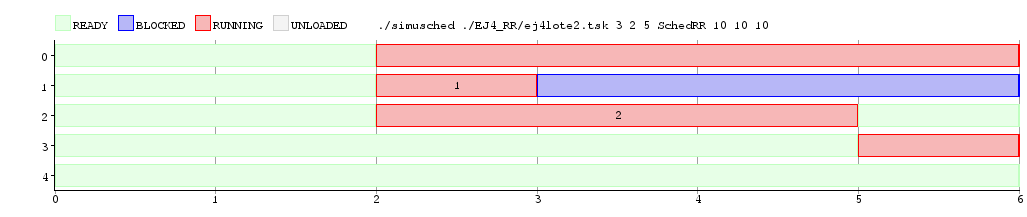
\includegraphics[width=450pt]{./EJ4_RR/ejercicio4-2lote3nucleo.png}
	{$Lote 2$ - Scheduler RR - 3 core}	
 \end{center}

 \indent Con este lote, además de lo observado anteriormente pudimos ver que, al tener una tarea bloqueada
 por un largo tiempo, el scheduler directamente la ignora.\\
 
\indent Luego de estos experimentos pudimos observar ciertos puntos del comportamiento del Round-Robin:\\
\begin{itemize}
\item  Carácter circular del algoritmo.
\item  Desalojo de las tareas cuando se bloquean o terminan y la inmediata asignación del núcleo a la siguiente tarea en caso de existir alguna.
\item  Libre de inanición.
\item  Una tarea bloqueada es ignorada por el scheduler hasta que se desbloquee.
\end{itemize}

\indent Finalmente, dado su carácter circular y equitativo, podemos afirmar que todas las tareas que 
estén en condiciones de correr serán ejecutadas y ninguna será negada de tiempo de procesamiento.\\


\subsubsection[Resolución Ejercicio 5]{Ejercicio 5}
\begin{center}
\textbf{PARTE 1}\\ 
\end{center}

\begin{center}
 \textbf{¿Qué problema están intentando resolver los autores?}
\end{center}

En el paper "Scheduling algorithms for multiprogramming
in a hard-real-time environment" los autores están intentando mostrar y resolver un problema que estaba surgiendo en esa época (1973). El uso de computadoras que controlaban y monitoreaban procesos industriales había empezado a incrementarse notablemente. Con esto aparecen los sistemas que tienen un "tiempo crítico" para procesar. Es decir, sistemas en donde el procesamiento estaba sujeto a un tiempo máximo al cual ejecutarse.\\
Por lo tanto necesitaban maximizar la eficiencia del uso del procesamiento, y para eso afirman que eso es posible mediante un algoritmo de schedulling que asegure procesar antes de ese tiempo crítico.\\
Por eso en el paper proponen dos algoritmos que manejan prioridades: prioridades fijas y dinámicas.\\

\begin{center}
 \textbf{¿Por qué introducen el algoritmo de la sección 7?\\¿Qué problema buscan resolver
 con esto?}
\end{center}

En la sección 7 introducen el algoritmo de prioridades dinamicas tratando de resolver un problema que muestra el algoritmo de prioridades fijas descripto en las secciones anteriores.\\
Al tener prioridades fijas, puede ocurrir inanición. Es decir, puede pasar que siempre lleguen tareas con prioridades más altas de las que se están por corriendo o por correr, dejándolas en espera y nunca atendiéndolas.\\
El algoritmo que presenta en esta sección tiene el nombre de "The deadline driven scheduling algorithm", explicando que se trata de un algoritmo que da más prioridad a las tareas en las que su deadline esté mas cercano. \\

\begin{center}
 \textbf{Explicar coloquialmente el significado del teorema 7}
\end{center}

El teorema 7 enuncia lo siguiente:\\

\textbf{For a given set of m task, the deadline driven scheduling algorithm is feasible if
and only if}
\begin{center}
 \[(C_{1}/T_{1})+(C_{2}/T_{2})+......+(C_{m}/T_{m}) \leq 1\]

\end{center}

Dicho teorema habla sobre la factibilidad y uso de las tareas en el algoritmo que 
se utilice como solución a la particular dificultad del algoritmo del scheduler fixed. \\
Puntualmente el lote de tareas m deberá cumplir una precondición en donde la 
suma de cada una de las relaciones entre el run time o tiempo de ejecución de la tarea, sobre el período de 
la misma de todas las tareas sea igual o menor a 1.\\

Esto quiere decir que el tiempo de ejecución de una tarea deberá ser considerablemente
menor al período de la misma para que el desarrollo y comportamiento del scheduler sea el deseado
y pudiese resolver la dificultad que se había generado por el anterior.\\

\begin{center}
 
\textbf{PARTE 2}\\

\end{center}
\hspace{3pt}
\begin{center}
\textbf{Algoritmo Scheduler Fixed - Explicación de Implementación}\\ 
\end{center}





Luego del estudio del Paper solicitado se realizo la implementación del dicho algoritmo,
utilizando una serie de estructuras para que este funcione acorde a lo pedido:

\begin{itemize}
 \item Un struct denominado  \textbf{tarea} el cual contiene el pid, el run\_time\_actual, periodo dandonos
 informacion de la tarea cargada.
 \item Una lista de $tarea$ nombrada \textbf{tareas}, esta es ordenada segun el periodo de las tareas
 de menor a mayor, obteniendo la prioridad del algoritmo.
  \item Una variable global \textbf{primera\_pasada} con la cual podemos realizar nuestra primer 
 comparacion de periodos entre tareas.
\end{itemize}

Ademas de estas estructuras utilizamos una funcion privada \textbf{insertarOrdenado} la cual como el
nombre lo dice va guardando en nuestra lista de tareas, las tareas a corde se van cargando en su
respectivo lugar comparando los periodos de las mismas.\\
De esta forma, la secuencia del algoritmo fue la siguiente:

\begin{enumerate}
 \item Llega una nueva tarea se la carga e inserta ordenadamente en la lista.
 \item La tarea corre hasta finalizar.
 \item Una vez que finaliza se chequea en la lista cual es la primera en orden de prioridad queda
 esta ready para correr.
 \end{enumerate}

De esta forma, con las estructuras y funciones logramos que nuestro scheduler trabaje de la forma
deseada.\\

Vale aclarar que, para que el scheduler funcione correctamente, es recomendable que los lotes de tareas
cumplan la factibilidad enunciada en el paper estudiado.\\


\hspace{3pt}
\begin{center}
\textbf{Algoritmo Scheduler Dynamic - Explicación de Implementación}\\ 
\end{center}

Una vez finalizado el estudio del paper, y habiendo notado las dificultades puntuales que enuncia el mismo
sobre el anterior Scheduler, se solicito desarrollar uno nuevo que solucione dichos problemas.\\

Para el desarrollo del mismo trabajamos con ciertas estructuras puntuales, las cuales enunciamos
a continuación:\\

\begin{itemize}
 \item Un struct denominado\textbf{tarea}  el cual contiene el pid, el run\_time\_actual, periodo y el deadline para tener
 informacion de la tarea cargada.
 \item Una lista de $tarea$ nombrada \textbf{tareas}, esta es ordenada segun el deadline de las tareas
 de menor a mayor, obteniendo la prioridad del algoritmo.
  \item Una variable global \textbf{primera\_pasada} con la cual podemos realizar nuestra primer 
 comparacion de periodos entre tareas.
\end{itemize}

Además de estas estructuras puntuales, definimos unas funciones de forma privada para poder
desarrollar el Scheduler en cuestión:

\begin{itemize}
 \item Función \textbf{insertarOrdenado}  
 \item Función  \textbf{chequearPeriodos}
  \end{itemize}
  
La función \textbf{insertarOrdenado}  como el nombre lo dice va guardando en nuestra lista $tareas$ las tareas
acorde van siendo cargadas respetando un orden, dicho orden se basa en la prioridad dada por los
deadline de las tareas. A menor deadline la tarea quedara en los primeros lugares de la lista.\\

La función \textbf{chequearPeriodos}, la cual revisa si la tarea que se encuentra al principio de la lista
tiene su deadline menor o igual a cero.\\

A partir de estas estructuras y funciones procedemos a explicar la secuencia de nuestro algoritmo:

\begin{enumerate}
 \item Llega una nueva tarea, se chequea si es la primera en llegar y en caso de no serlo se la inserta ordenadamente.
 \item Empieza a correr una tarea, y en cada Tick de reloj del cpu se va disminuyendo en uno el periodo y deadline
 de todas las demas tareas que no estan corriendo, mientras que la que se encuentra ejecutando
 se le disminuye en uno su run\_time y su periodo.
 \item En caso de que nuestra función booleana $chequearPeriodos$ de True en un tick de reloj
 y la tarea que este corriendo no haya finalizado esta sera desalojada guardando su run\_time actual y su deadline
 insertandola ordenadamente en la lista para que luego pueda finalizar su ejecución.
 \item Si $chequearPeriodos$ no dio nunca True durante la ejecución de la tarea, esta podra finalizar sin
 inconvenientes y posteriormente se cargará la primer tarea de la lista en orden de prioridad.
\end{enumerate}

De esta forma, nuestro Scheduler continua hasta finalizar todas las tareas manteniendo esta secuencia.\\

Vale aclarar, como en el anterior algoritmo, que para un correcto funcionamiento de nuestro
Scheduler es recomendable que el lote de tareas a utilizar cumpla la factibilidad enunciada
en el paper.\\

\newpage

\section{Parte 3: Evaluando los algoritmos de scheduling}


\subsection{Ejercicios}
\begin{itemize}
 
\item \textbf{Ejercicio 6}  Programar un tipo de tarea TaskBatch que reciba dos parametros: total cpu y
cant bloqueos. Una tarea de este tipo debera realizar cant bloqueos llamadas bloqueantes, en
momentos elegidos pseudoaleatoriamente. En cada tal ocasion, la tarea debera permanecer
bloqueada durante exactamente un (1) ciclo de reloj. El tiempo de CPU total que utilice una
tarea TaskBatch debera ser de total cpu ciclos de reloj (incluyendo el tiempo utilizado para
lanzar las llamadas bloqueantes; no ası el tiempo en que la tarea permanezca bloqueada).

\item \textbf{Ejercicio 7} Elegir al menos dos metricas diferentes, definirlas y explicar la semantica de
su definicion. Diseñar un lote de tareas TaskBatch, todas ellas con igual uso de CPU, pero
con diversas cantidades de bloqueos. Simular este lote utilizando el algoritmo SchedRR y una
variedad apropiada de valores de quantum. Mantener fijo en un (1) ciclo de reloj el costo de
cambio de contexto y dos (2) ciclos el de migracion. Deben variar la cantidad de nucleos de
procesamiento. Para cada una de las metricas elegidas, concluir cual es el valor optimo de
quantum a los efectos de dicha metrica.

\item \textbf{Ejercicio 8} Implemente un scheduler Round-Robin que no permita la migracion de procesos
entre nucleos (SchedRR2). La asignacion de CPU se debe realizar en el momento en que se produce la carga 
de un proceso (load). El nucleo correspondiente a un nuevo proceso sera aquel
con menor cantidad de procesos activos totales (RUNNING + BLOCKED + READY). Diseñe y realice un conjunto 
de experimentos que permita evaluar comparativamente las dos implementaciones de Round-Robin.

\item \textbf{Ejercicio 9} Disenar un lote de tareas cuyo scheduling no sea factible para el algoritmo de
prioridades fijas pero sı para el algoritmo de prioridades dinamicas.

\item \textbf{Ejercicio 10} Disenar un lote de tareas, cuyo scheduling sı sea factible con el algoritmo de
prioridades fijas, donde se observe un mejor uso del CPU por parte del algoritmo de prioridades
dinamicas.
\end{itemize}
\subsection{Resultados y Conclusiones}

\subsubsection[Resolución Ejercicio 6]{Ejercicio 6}

\indent Al igual que con la tarea TaskConsola, mencionaremos nuestro implementación y acontinuación de la misma 
explicaremos ciertos puntos de la misma.\\
 \begin{verbatim}
                       void TaskBatch(int pid, vector<int> params) {
                            int total_cpu = params[0];
                            int cant_bloqueos = params[1];
                            srand(time(NULL));
                            vector<bool> uso = vector<bool>(total_cpu);
                            for(int i=0;i<(int)uso.size();i++) 
                               uso[i] = false;
	                       for(int i=0;i<cant_bloqueos;i++) {
                                   int j = rand()%(uso.size());
                                   if(!uso[j])
                                      uso[j] = true;
                                   else
                                      i--; 
                                   }
                            for(int i=0;i<(int)uso.size();i++) {
                                if( uso[i] )
                                    uso_IO(pid,1); 
                                else
                                    uso_CPU(pid, 1); 
                               }
                            }
 \end{verbatim}

 \indent Para este tipo de tarea, creamos un vector de tamaño igual a $total_cpu$ el cual tendra bool, ya sea true o false
 dependiendo del uso que se le de dentro de la tarea, ya sea uso\_IO o uso\_CPU. En caso de ser uso\_IO sera true, y sino false.\\
 Luego, utilizaremos un ciclo que ira desde 0 hasta el tamaño del vector y dependiendo el valor booleano, usará la funciones
 dadas por la catedra uso\_IO o uso\_CPU.\\
 
 \subsubsection[Resolución Ejercicio 7]{Ejercicio 7}
 Las métricas elegidas fueron:
\begin{itemize}
 \item \textbf{Turnaround}: Es el intervalo de tiempo desde que un proceso es cargado hasta que este finaliza su ejecución.
 \item \textbf{Waiting Time}: Es la suma de los intervalos de tiempo que un proceso estuvo en la cola de procesos $ready$.
\end{itemize}

\indent \indent Como las tareas TaskBatch se bloquean pseudoaleatoriamente, 
para obtener datos relevantes tomamos un promedio de las mediciones.\\
\indent A la hora de encarar la experimentación, lo que realizamos trabajar con
varios quantum distintos para poder obtener una mejor apreciacion 
del efecto del $quantum$ en la ejecución de este tipo de tareas. 

\indent A partir de este resultado, desarrollamos los siguientes gráficos de turnaround time 
en función del quantum, utilizando 2 y 3 núcleos

\indent Luego de realizar mediciones con distintos $quantum$,
tomamos la decisión de trabajar con los mismos $quantum$ para cada nucleo
al trabajar con más de 1 core. Igualmente, mostraremos a continuacion un grafico
ejemplificando la diferencia que se produce al trabajar con distintos $quantums$ por
core.\\

\begin{center}
    	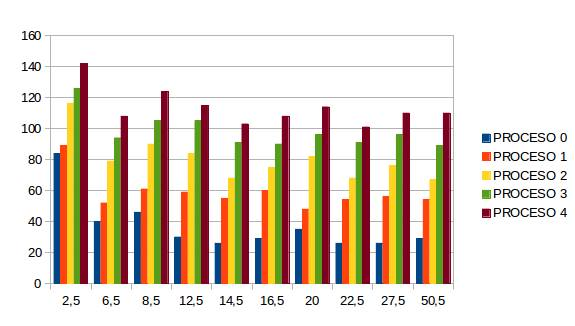
\includegraphics[width=1\textwidth]{./EJ7/turnarounddistquan.png}
	{Turnaround - 2 core - Prueba Quantum distintos por Core}\\
	{$Eje X = Quantum; $\\$ Eje Y = Tiempo$}\\
 \end{center}

\indent Al realizar este gráfico y varias mediciones con distintos $quantum$ 
por core, observamos que no eran mediciones rigurosas, 
ya que una proceso podria estar corriendo con distintos tiempos por la
migracion de procesos por core.\\

 \indent Por consiguiente, al trabajar con las nuevas mediciones, 
 concluimos con 2 hipotesis:
 
 \begin{itemize}
  \item Con 2 nucleos las mediciones de tiempo tienden a estabilizarse a partir de un $quantum$ igual a 9.
  \item Con 3 nucleos las mediciones de tiempo tienden a estabilizarse a partir de un $quantum$ igual a 11.
 \end{itemize}
 \begin{center}
 \textbf{Turnaround Time} 
  \end{center}

 \begin{center}
 \textbf{2 Core}
 \end{center}
  A continuación se muestran los Diagramas de Gantt más relevantes:
  
  \begin{center}
    	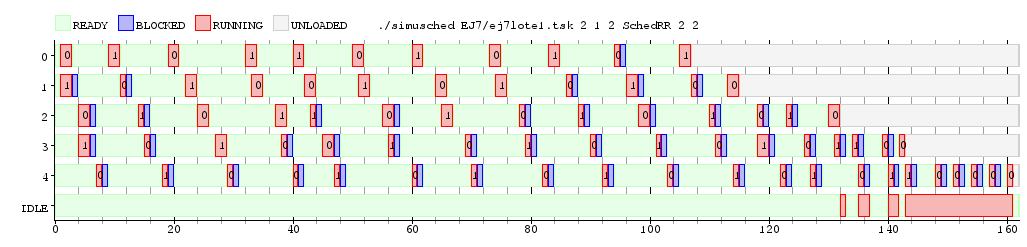
\includegraphics[width=450pt]{./EJ7/ej7tour2core1quan.png}
	{$Lote 1$ - Turnaround - 2 core - Quantum igual a 2}	
 \end{center}

   \begin{center}
    	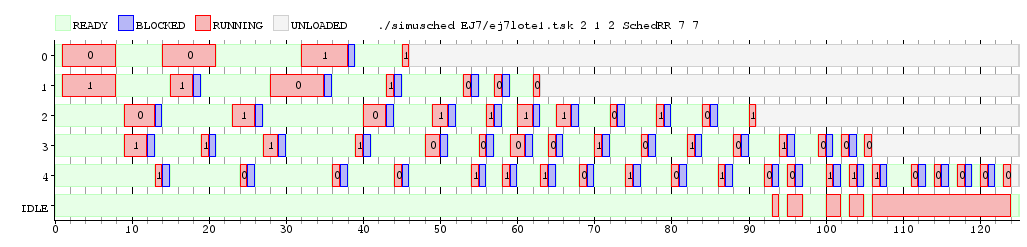
\includegraphics[width=450pt]{./EJ7/ej7tour2core3quan.png}
	{$Lote 1$ - Turnaround - 2 core - Quantum igual a 7}	
 \end{center}
 
 
 \indent La performance empieza a mejorar a medida que el $quantum$ aumenta.
 
   \begin{center}
    	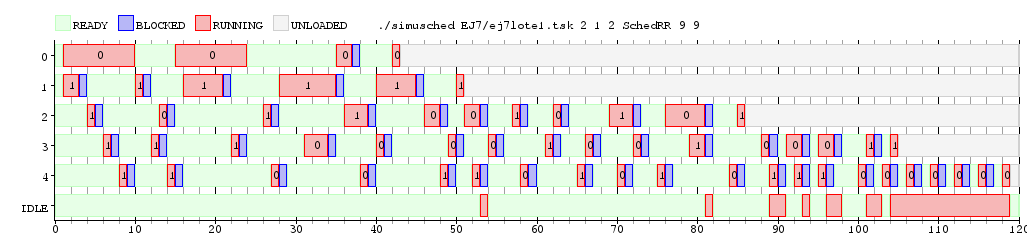
\includegraphics[width=450pt]{./EJ7/ej7tour2core4quan.png}
	{$Lote 1$ - Turnaround - 2 core - Quantum igual a 9}	
 \end{center}

  
   \indent La performance sigue mejorando,a partir de este valor, el desempeño 
   comienza a estabilizarse, como muestran los siguiente dos gráficos. 
   
   Las pequeñas diferencias en los valores se deben a que este tipo de tarea presenta
   una pseudoaleatoridad notoria.\\
  
   \begin{center}
    	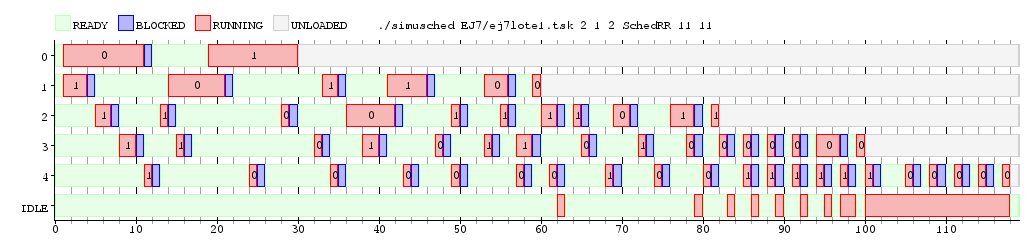
\includegraphics[width=450pt]{./EJ7/ej7tour2core5quan.png}
	{$Lote 1$ - Turnaround - 2 core - Quantum igual a 11}	
 \end{center}
 

    \begin{center}
    	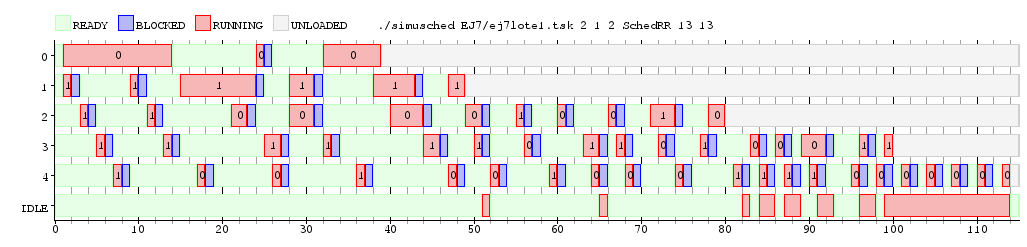
\includegraphics[width=450pt]{./EJ7/ej7tour2core8quan.png}
	{$Lote 1$ - Turnaround - 2 core - Quantum igual a 13}	
 \end{center}

 \indent Como mencionamos, las mediciones tienden a estabilizarse con un $quantum$ 
 igual a 9, pero la mejor performance obtenida es con un $quantum$ igual a 13,
 teniendo en cuenta como mencionamos la pseudoaleatoridad de este tipo de tarea.\\
 \indent Se puede observar en la primer figura que a pesar de trabajar con 2 cores, 
 al tener un quantum bajo (igual a 2)  el costo es alto.
  
   \begin{center}
    	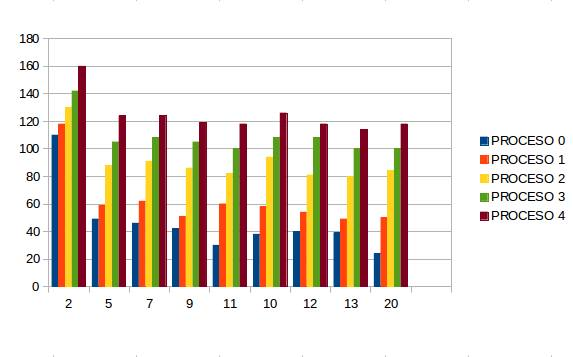
\includegraphics[width=1\textwidth]{./EJ7/tour2core.png}
	{Turnaround - 2 core}	\\
	{$Eje X = Quantum$\\$ Eje Y = Tiempo$}\\
 \end{center} 
 
 \begin{center}
  \textbf{Waiting Time}
 \end{center}

  \begin{center}
    	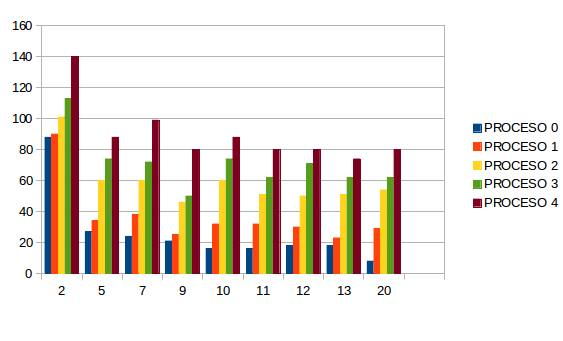
\includegraphics[width=1\textwidth]{./EJ7/waiting2core.jpg}
	{Waiting Time - 2 core}	\\
	{$Eje X = Quantum$\\$Eje Y = Tiempo$}\\
 \end{center} 
 
 \indent Con este tipo de metrica, se comienza a estabilizar a partir del $quantum$ igual
 a 5, obteniendo su mejor  performance con el $quantum$ igual a 13.\\
 
   \begin{center}
   \textbf{3 Core}
   \end{center}
   \indent A continuación, al igual que con 2 cores, mostraremos los resultados mas relevantes:
   
   \begin{center}
    	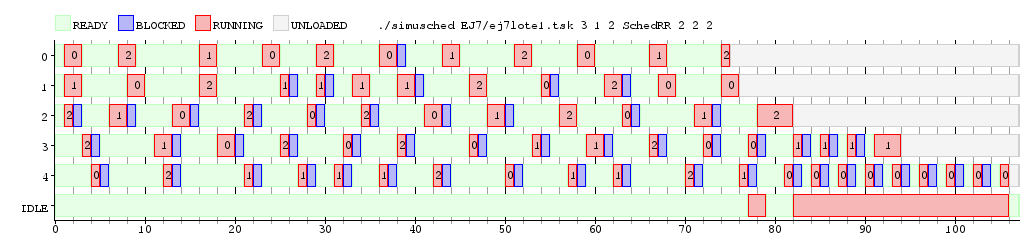
\includegraphics[width=450pt]{./EJ7/ej7tour3core1quan.png}
	{$Lote 1$ - Turnaround - 3 core - Quantum igual a 2}	
 \end{center}

 \indent Se observa que al tener otro core mas,a diferencia de con 2, 
 a pesar de estar con un $quantum$ bajo, la performance va en alto.\\ 
 
   \begin{center}
    	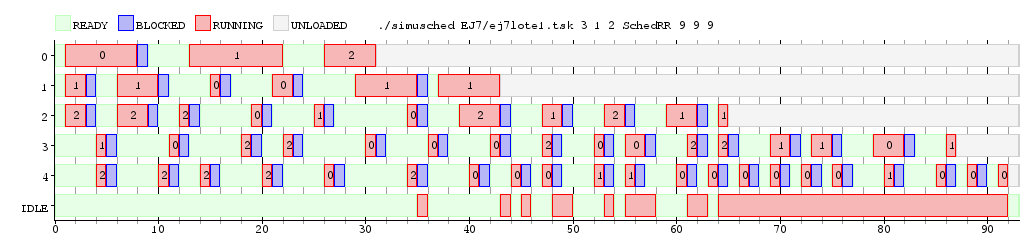
\includegraphics[width=450pt]{./EJ7/ej7tour3core4quan.png}
	{$Lote 1$ - Turnaround - 3 core - Quantum igual a 9}	
 \end{center}
 
 
 \indent La performance empieza a mejorar a medida que el $quantum$ aumenta.
 
   \begin{center}
    	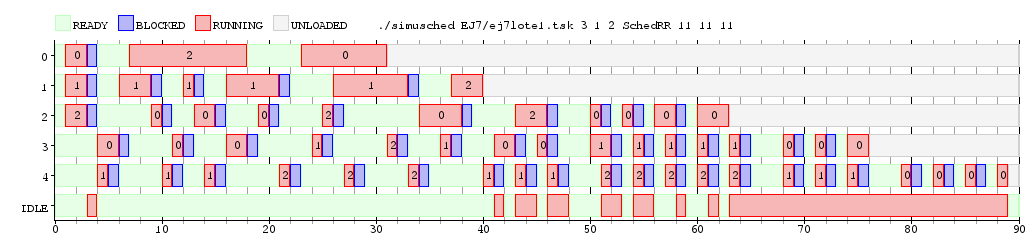
\includegraphics[width=450pt]{./EJ7/ej7tour3core5quan.png}
	{$Lote 1$ - Turnaround - 3 core - Quantum igual a 11}	
 \end{center}
  
   \begin{center}
    	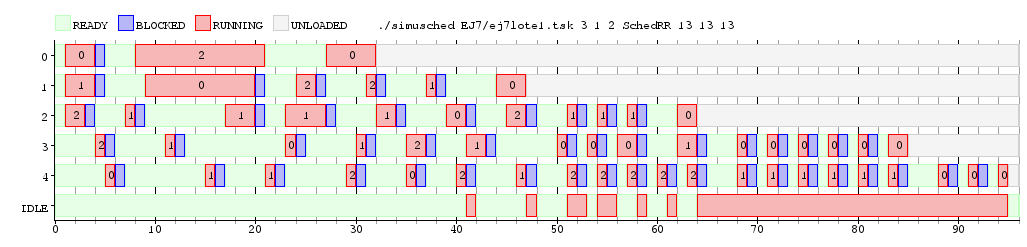
\includegraphics[width=450pt]{./EJ7/ej7tour7core6quan.png}
	{$Lote 1$ - Turnaround - 3 core - Quantum igual a 13}	
 \end{center}
 
 \begin{center}
    	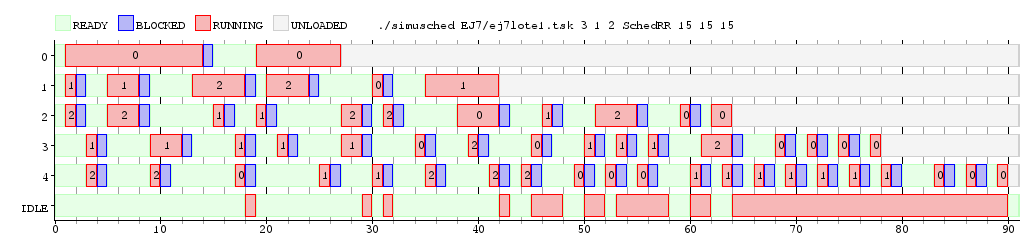
\includegraphics[width=450pt]{./EJ7/ej7tour8core6quan.png}
	{$Lote 1$ - Turnaround - 3 core - Quantum igual a 15}	
 \end{center}
 
 \indent A diferencia que en nuestra hipótesis conjeturada para con dos cores, 
 con un $quantum$ igual a 11 se obtiene la mejor  performance, 
 pero teniendo en cuenta el tipo de tarea con la 
 que se estuvo trabajando, a partir del $quantum$ igual a 9 ya se estabiliza notoriamente.\\
   
    \begin{center}
    	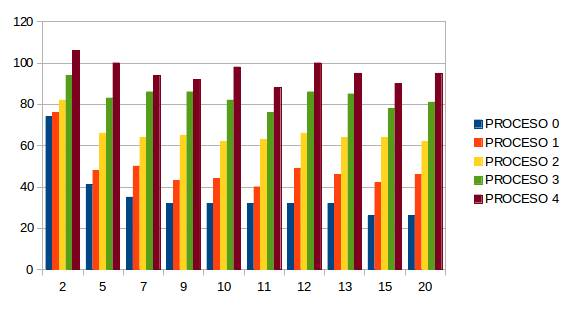
\includegraphics[width=1\textwidth]{./EJ7/tour3core.png}
	{Turnaround - 3 core}\\
	{$Eje X = Quantum $\\$ Eje Y = Tiempo$}\\
 \end{center} 
  
   \begin{center}
  \textbf{Waiting Time}
 \end{center}

  \begin{center}
    	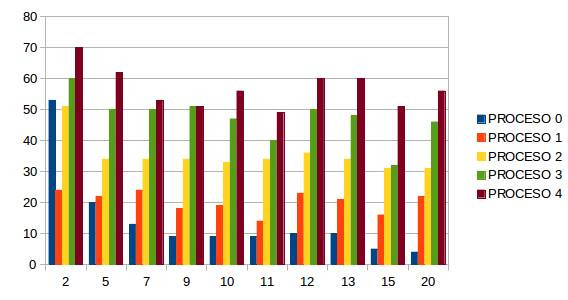
\includegraphics[width=1\textwidth]{./EJ7/waintin3core.jpg}
	{Waiting Time - 3 core}	\\
	{$Eje X = Quantum $\\$Eje Y = Tiempo$}\\
 \end{center} 
 
   \indent Con este tipo de metrica,se obteniene a diferencia de con Turnaround  
   su mejor performance con el $quantum$ igual a 15.\\
  
 \begin{center}
  \textbf{Conclusiones}
 \end{center}


\indent \indent La diferencia entre los valores de quantum entre los casos 
se puede presumir a que cada vez que agregamos un núcleo aumentamos 
la posibilidad de una migración de la tareas.\\
\indent \indent En todos lo casos se observa la influencia negativa que proviene 
de elegir un quantum con valores pequeños.\\
\indent \indent Agregar núcleos de procesamiento mejora significativamente 
la performance de acuerdo a la métricas con las que
trabajamos, al permitir más procesamiento en pararelo y disminuyendo 
los waiting time de las tareas.\\
\indent \indent  Fijada una cantidad de núcleos puntual, aumentar el valor del
quantum también mejora la performance, igualmente, como vimos, a partir de cierto valor 
de quantum, las mejoras en la performance tienden a estabilizarse y dejan de ser 
muy significativas. 
Esto se produce a que las tareas con mas cantidad de bloqueos en 
algun momento dejan de consumir todo el quantum otorgado si este es aumentado en su valor. 
 
 
 
\subsubsection[Resolución Ejercicio 8]{Ejercicio 8}
La idea principal de esta nueva version de $Round-Robin$ se centraliza en que no permita migracion entre
cores, esto se basa principalmente en utilizar una cola para cada nucleo por separado, y en cada
cola respectiva se encolaran las tareas que fueron asignadas inicialmente a cada nucleo.\\
Para desarrollar este tipo de algoritmo, el cual denominaremos $RR2$, utilizamos estructuras
puntuales, enunciadas a continuacion:\\
\begin{itemize}
 \item Un vector $quantum$ y otro $quantumActual$, los cuales siguen cumpliendo la misma funcion que
 en Round-Robin 1.
 \item Un vector de colas denominado $colas$, en el cual la posicion $i$ encontraremos la cola correspondiente
 a ese nucleo de procesamiento.
 \item Un diccionario de $Bloqueados$, donde la clave contendra el numero de core, y en definicion
 la tareas bloqueadas de ese core. Esto nos beneficiara cuando haya que reubicarla en la cola de procesos ready.
 \item Un vector de enteros $cantidad$, que como la palabra lo define, tendra en cada posicion $i$ 
 la totalidad de las tareas, ya sea bloqueadas, activas o en estado ready que tiene asignado ese core, beneficiandonos
 la determinacion del nucleo al que se asignara la tarea al momento de cargarla.
\end{itemize}
Cuando se carga una tarea, previamente, se chequeara que core tiene menor cantidad de procesos totales asignados (
aqui es donde el vector $cantidad$ entra en juego). Una vez que se obtiene este nucleo, se agrega 
la tarea a la cola correspondiente y se actualiza la cantidad sumando una unidad.\\
\indent Al bloquearse un proceso, se define una nueva entrada en el diccionario $bloqueados$ con el
pid y el nucleo correspondiente. De esta forma, al desbloquearse, colocamos la tarea en la cola del core
correspondiente y eliminamos la entrada del diccionario. Así logramos resolver el inconveniente de la nula
migracion entre nucleos.\\
\indent Finalmente, cuando una tarea finaliza, la quitamos y descontamos una unidad a la posicion $i$ del vector
$cantidad$. Esta es la unica vez, en la cual se descuenta. Aunque una tarea se bloquee, la misma
seguira contando en el vector. De esta forma se cumplira, que las tareas son asignadas a los cores
con menor cantidad de tareas.\\
Luego de realizar dicha implementacion, en comparacion al Round-Robin original, hemos conjeturado 
las siguientes hipotesis:

\begin{enumerate}
 \item Dados un mismo lote de tareas y una misma configuracion del scheduler (mismos costo en cambio
de contexto y quantum) un unico nucleo de procesamiento, ambos algoritmos deben comportarse
de la misma manera.
\item Comportamiento menos eficiente en el RR2 con respecto al paralelismo, ya que al no permitir
migracion de nucleos este lo pierde.
\item Comportamiento mas eficiente en el RR2 con lotes de tareas que se bloquean un gran numero
de veces. Esto surge ya que el Round-Robin original, es mas proclive a realizar cambios de contexto con la posibilidad
de darse un cambio de core.
\end{enumerate}

Por consiguiente, procederemos a demostrar lo conjeturado.\\

Iniciando con nuestra primer conjetura:\\

\textbf{Dados un mismo lote de tareas y una misma configuracion del scheduler 
 (mismos costo en cambio de contexto y quantum)
un unico nucleo de procesamiento, ambos algoritmos deben comportarse
de la misma manera.}\\

Trabajando con el lote que mencionamos a continuacion:
    
    \begin{verbatim}
                                     TaskCPU 70
                                     TaskConsola 2 4 5
                                     TaskCPU 40
                                     TaskConsola 3 2 3
                                     TaskCPU 30
    \end{verbatim}

Utilizando un $quantum$ igual a 5 y un cambio de contexto igual a 1 obtuvimos 
resultados muy marcados, viendose notoriamente lo que queremos demostrar.\\

\begin{center}
    	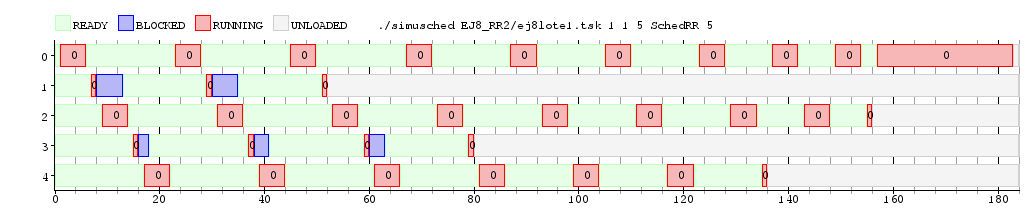
\includegraphics[width=450pt]{./EJ8_RR2/dif1corerr.png}
	{$Lote 1$ - Round Robin - 1 core - Quantum = 5 - cambio de contexto = 1}	
 \end{center}
 
 \begin{center}
    	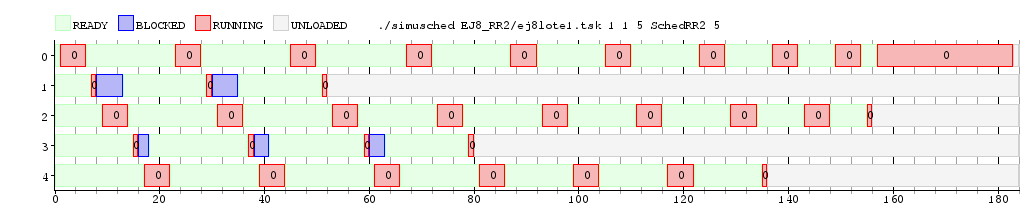
\includegraphics[width=450pt]{./EJ8_RR2/dif1corerr2.png}
	{$Lote 1$ - Round Robin 2 - 1 core - Quantum = 5 - cambio de contexto = 1}	
 \end{center}

Continuando con un lote distinto para ser mas precisos:

 \begin{verbatim}
                                     TaskCPU 70
                                     TaskConsola 5 6 7
                                     TaskCPU 40
                                     TaskConsola 10 9 8
                                     TaskCPU 30
 \end{verbatim}
 
Llegamos a lo siguiente:\\

 \begin{center}
    	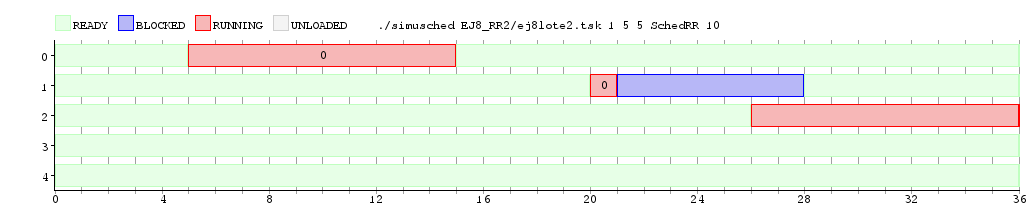
\includegraphics[width=450pt]{./EJ8_RR2/dif2corerr.png}
	{$Lote 2$ - Round Robin - 1 core - Quantum = 10 - cambio de contexto = 5}	
 \end{center}
 
 \begin{center}
    	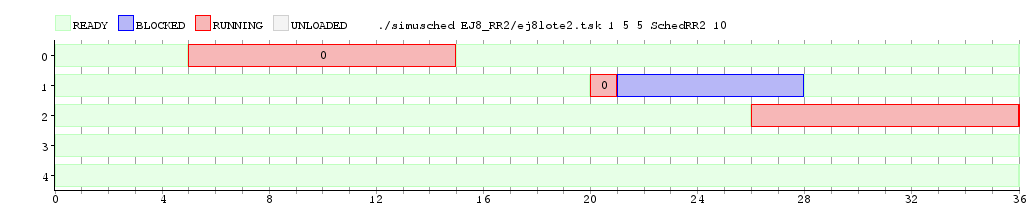
\includegraphics[width=450pt]{./EJ8_RR2/dif2corerr2.png}
	{$Lote 2$ - Round Robin 2 - 1 core - Quantum = 10 - cambio de contexto = 5}	
 \end{center}
 
 Viendose nuevamente, la igualdad que mencionamos. Hemos podido ver a su vez, que la unica
 forma en la que los resultados sean distintos con el mismo lote seria modificando o la
 cantidad de $quantum$ o la unidad de cambio de contexto entre uno y otro.\\
 
 Aqui, un ejemplo para mayor precision:\\
 
  \begin{center}
    	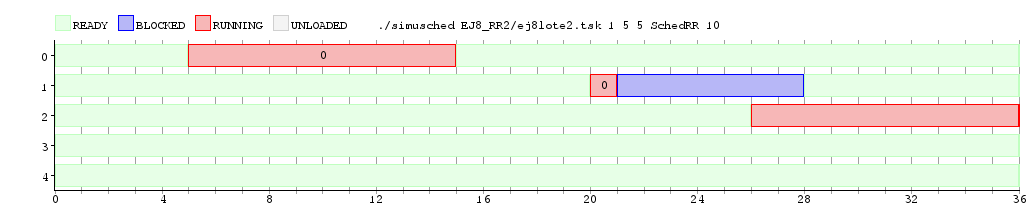
\includegraphics[width=450pt]{./EJ8_RR2/dif3corerr.png}
	{$Lote 2$ - Round Robin - 1 core - Quantum = 10 - cambio de contexto = 5}	
 \end{center}
 
 \begin{center}
    	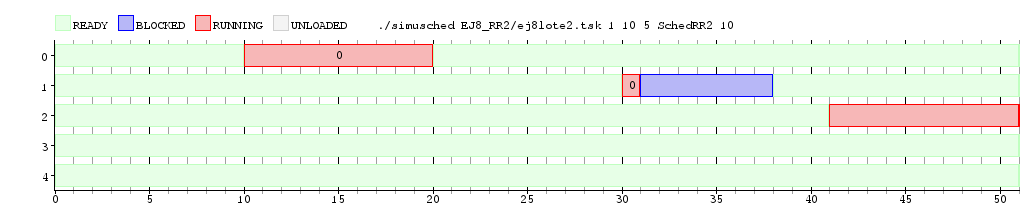
\includegraphics[width=450pt]{./EJ8_RR2/dif3corerr2.png}
	{$Lote 2$ - Round Robin 2 - 1 core - Quantum = 10 - cambio de contexto = 10}	
 \end{center}
 
 Concluimos entonces que, al trabajar con colas globales o no, utilizando un unico nucleo y
 mismo lote quantum y cambio de contexto, ambos schedulers se comportan de la misma
 manera.\\
 
 Procedemos a demostrar la segunda conjetura:\\
 
 \textbf{Comportamiento menos eficiente en el RR2 con respecto al paralelismo, ya que al no permitir
migracion de nucleos este lo pierde}\\

Para demostrar esta conjetura trabajamos con procesos que demanden mas uso del cpu como 
lo son las $taskCPU$\\

Un ejemplo de los lotes utilizados fue el siguiente:\\

\begin{verbatim}
                                     TaskCPU 40
                                     TaskCPU 15
                                     TaskCPU 50
                                     TaskCPU 30
                                     TaskCPU 50
\end{verbatim}

Obteniendo los siguientes datos relevantes:\\

\begin{center}
    	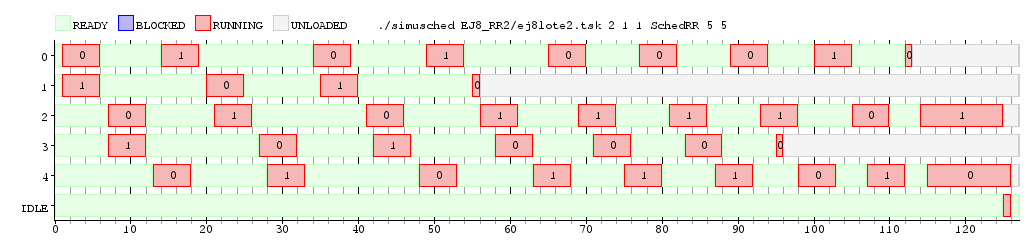
\includegraphics[width=450pt]{./EJ8_RR2/dif10corerr.png}
	{$Lote 3$ - Round Robin - 2 core - Quantum = 5 - cambio de contexto = 1}	
 \end{center}
 
 \begin{center}
    	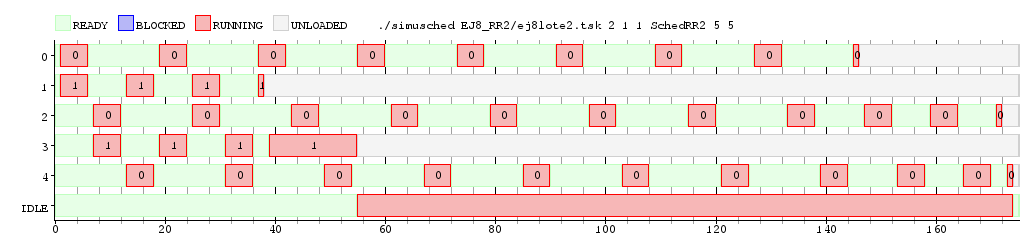
\includegraphics[width=450pt]{./EJ8_RR2/dif10corerr2.png}
	{$Lote 3$ - Round Robin 2 - 2 core - Quantum = 5 - cambio de contexto = 1}	
 \end{center}
 
 Se puede ver en estos diagramas como la implementacion del Round Robin original trabaja
 mejor finalizando la ejecución de las tareas hasta 50 milisegundos antes.\\
 Esto se da por la falta de paralelismo de el RR2 ya que al ser asignados los procesos
 a cada core, cuando uno de los dos finaliza, este queda ocioso ya que no existe la
 posibilidad de migrar  procesos.\\
 
 Por ultimo, nuestra tercer y ultima conjetura:\\
 
 \textbf{Comportamiento mas eficiente en el RR2 con lotes de tareas que se bloquean un gran numero
de veces}

Para esta conjetura, trabajamos con lotes de tareas que utilicen el CPU y se bloqueen muchas
veces para poder demostrar la mejor performance del RR2.\\

A continuacion un ejemplo, con el siguiente lote:

\begin{verbatim}
                                     TaskCPU 40
                                     TaskBatch 10  5
                                     TaskCPU 50
                                     TaskBatch 15 8
                                     TaskCPU 10

\end{verbatim}


   \begin{center}
    	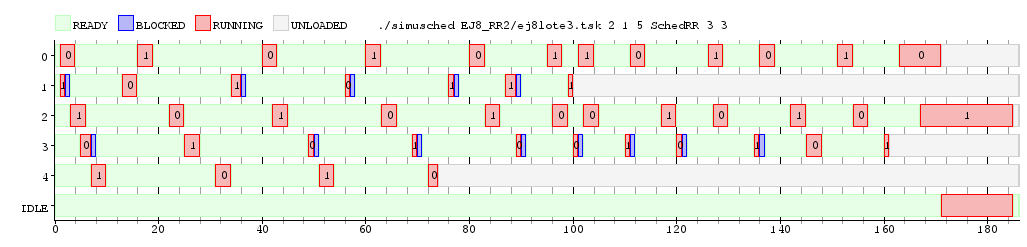
\includegraphics[width=450pt]{./EJ8_RR2/dif5corerr.png}
	{$Lote 3$ - Round Robin - 2 core - Quantum = 3 - cambio de contexto = 1}	
 \end{center}
 
 \begin{center}
    	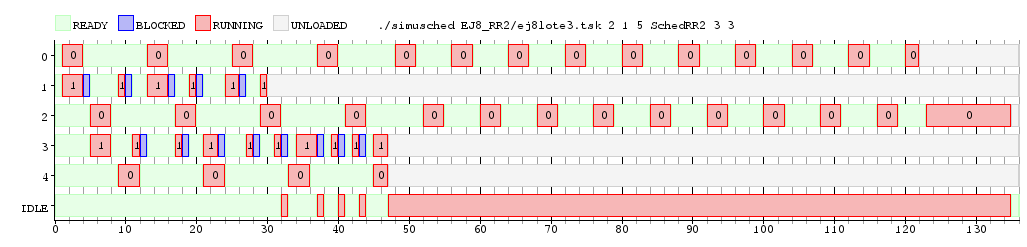
\includegraphics[width=450pt]{./EJ8_RR2/dif5corerr2.png}
	{$Lote 3$ - Round Robin 2 - 2 core - Quantum = 3 - cambio de contexto = 1}	
 \end{center}

 Se puede observar por los diagramas como el RR2 tiene una mejor performance en este estilo
 de lotes llegando a finalizar las ejecuciones hasta 50 milisegundos antes que el Round-Robin
 original.\\
 Como para el Round-Robin original tiene perdida de tiempo con el cambio de contexto y
 migracion de tareas este empeora su performance en comparacion al RR2 que no admite
 este tipo de migracion es notorio la superioridad en relacion a nuestra conjetura.\\
 
 Podemos concluir luego de estas demostraciones que, el Round-Robin original es ampliamente
 superior desde el punto de vista de la performance que obtiene al trabajar con tareas
 que demanden mucho uso del CPU, mientras que el RR2 sera mejor para cuando se utilicen
 tareas que se bloqueen por un tiempo considerable.\\
 
 


  
\subsubsection[Resolución Ejercicio 9]{Ejercicio 9}

\subsubsection[Resolución Ejercicio 10]{Ejercicio 10}

\newpage


%%%%%%%%%%%%%%%%%%%%%%%%%%%%%%%%%%%%%%%%%%%%%%%%%%%%%%%%%%%%%%%%%%%%%%%%%%%%%%%
%% Conclusión                                                                %%
%%%%%%%%%%%%%%%%%%%%%%%%%%%%%%%%%%%%%%%%%%%%%%%%%%%%%%%%%%%%%%%%%%%%%%%%%%%%%%%

\newpage
\section{Bibliografía}

\begin{itemize}
 \item Cátedra de Sistemas Operativos - Clases teóricas y prácticas (1º Cuatrimestre 2015)
 \item Facultad de Ingenieria Uruguay \\
 $(https://eva.fing.edu.uy/pluginfile.php/75120/mod\_resource/content/1/6-SO-Teo-Planificacion.pdf)$
 \item Operating Systems Concepts, Abraham Silberschatz \& Peter B. Galvin
\end{itemize}

\end{document}
